\chapter{Configureren van uw MEGA65}

\section{Configureren van uw MEGA65}
\label{cha:configuringyourmega}
\index{Configuratie}

Dit hoofdstuk beschrijft hoe u uw MEGA65 configureert.

Omdat de configuratiegegevens op de SD-kaart worden opgeslagen, beschrijft dit hoofdstuk ook hoe u een nieuwe SD-kaart voorbereidt. Uw MEGA65 wordt met een vooraf geïnstalleerde SD-kaart geleverd. Indien u uw MEGA65 met de vooraf geïnstalleerde SD-kaart configureert en later een nieuwe SD- of microSD-kaart installeert, moet u uw configuratie-instellingen opnieuw instellen.

Dit hoofdstuk laat u tevens kennismaken met de website MEGA65 Filehost, waarmee u games, apps, hulpprogramma's en systeemupdates voor uw computer kunt downloaden.

\section{Configuratiehulpprogramma}
\label{sec:configuration-utility}
\index{Configuratie!Hulpprogramma}

U kunt uw MEGA65 configureren met het Configuratiehulpprogramma. Dit omvat de instellingen die werden weergegeven toen u de computer voor het eerst inschakelde en vele andere.

Om het Configuratiehulpprogramma te openen, schakelt u de MEGA65 uit, houdt u de toets \specialkey{ALT} ingedrukt en schakelt u de MEGA65 weer in. Het hulpprogrammamenu\index{Hulpprogrammamenu} verschijnt met verschillende opties. Druk op \megakey{1} om het Configuratiehulpprogramma te starten.

\begin{center}
  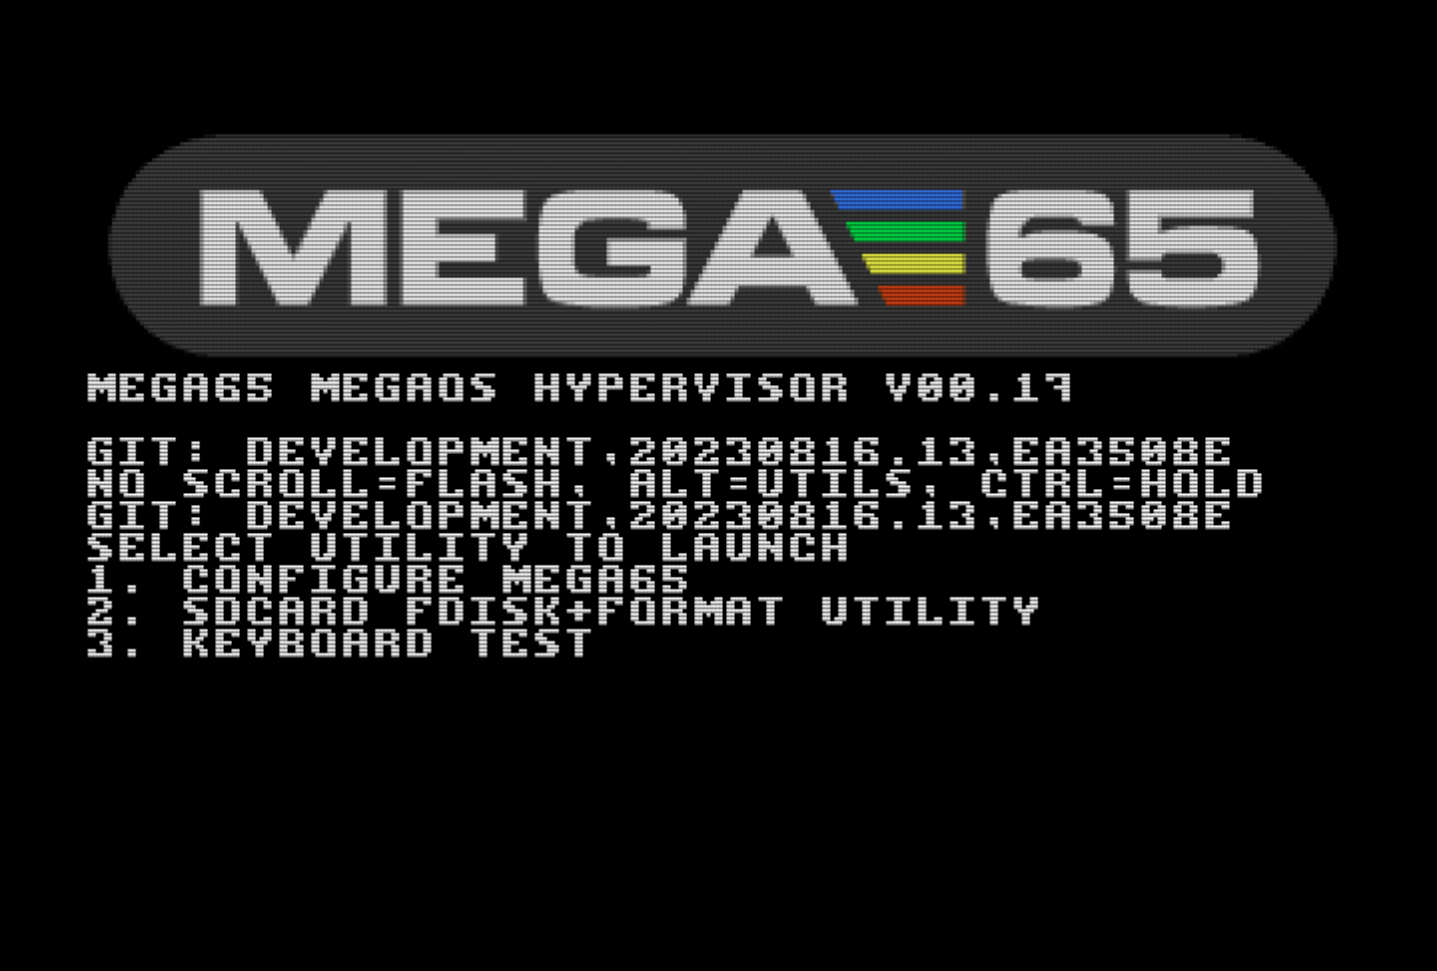
\includegraphics[width=0.7\linewidth]{images/ss-utilmenu.png}
\end{center}

Het Configuratiehulpprogramma bevat verscheidene bladzijden met instellingen, die u kunt doorlopen met het toetsenbord of met een op poort 1 aangesloten muis. Gebruik \megakey{$\leftarrow$} en \megakey{$\rightarrow$} om tussen de bladzijden te bladeren en \megakey{$\uparrow$} en \megakey{$\downarrow$} om onderdelen op een bladzijde te selecteren. Druk op \specialkey{RETURN} of \megakey{SPACE} om een instelling om te schakelen of een waarde te wijzigen.

\subsection{Input}
\index{Configuratie!Muis}

Op de bladzijde {\bf Input} stelt u de muisinstellingen voor de twee randapparaatpoorten in.

\begin{center}
  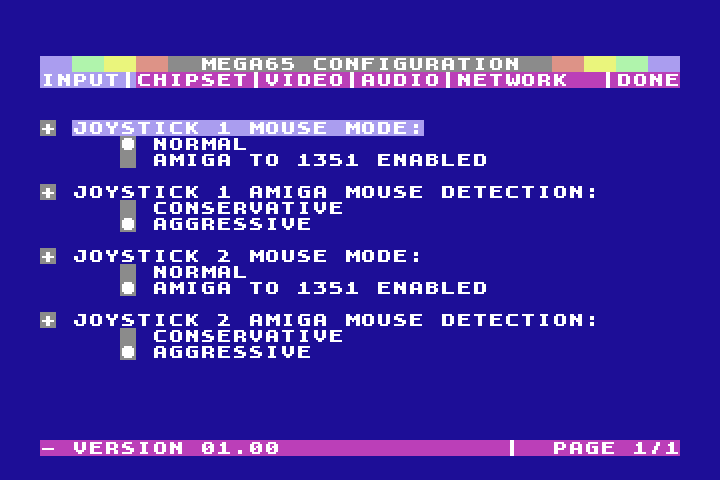
\includegraphics[width=0.7\linewidth]{images/ss-m65config-1.png}
\end{center}

De MEGA65 ondersteunt de Commodore 1351-muis,\index{Commodore 1351-muis} de Commodore Amiga-muis\index{Commodore Amiga-muis} of moderne equivalenten, zoals een USB-muis die met een \href{https://retrohax.net/shop/amiga/mouster/}{mouSTer}-adapter is aangesloten.\index{mouSTer-adapter} De poort moet op het juiste muistype worden ingesteld, waarbij {\bf normal} naar de 1351-muis verwijst. Indien een Amiga-muis is aangesloten terwijl de poort in de modus {\bf normal} staat, kan deze het gedrag van het toetsenbord verstoren.

Met de instelling {\bf 1351 De-jitter} stelt u de gevoeligheid in de Commodore 1351-muismodus af om jitter van het muispijltje te voorkomen. Het wordt aanbevolen deze op {\bf on} te laten staan wanneer u in de modus {\bf normal} een 1351-muis gebruikt.

\subsection{Chipset}
\index{Configuratie!Opstartschijf}

Op de bladzijde {\bf Chipset} stelt u verschillende functies in, waaronder de real-time klok.

\begin{center}
  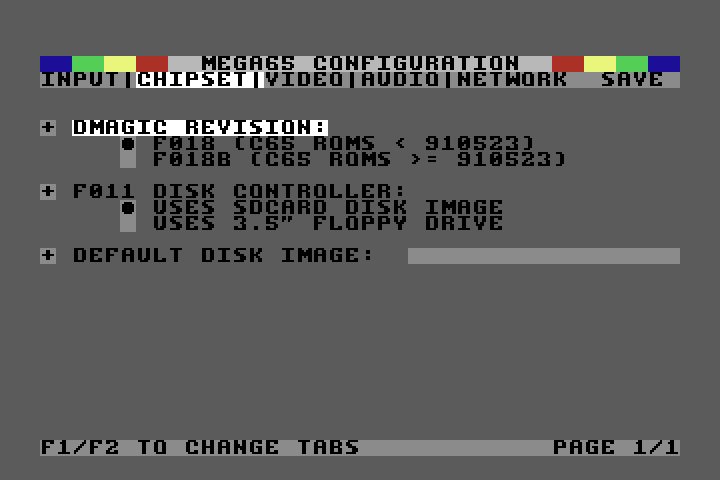
\includegraphics[width=0.7\linewidth]{images/ss-m65config-2.png}
\end{center}

Om de real-time klok in te stellen, selecteert u het tijd- of datumveld, typt u de volledige waarde en drukt u vervolgens op \specialkey{RETURN}.\index{Real-time klok!Datum/tijd instellen}\index{Configuratie!Real-time klok} De klokinstelling wordt pas van kracht wanneer u op \specialkey{RETURN} drukt; zonder \specialkey{RETURN} wijzigt er niets. Merk op dat alle overige instellingen pas aan het einde worden opgeslagen. Alleen de RTC wordt onmiddellijk bijgewerkt.

Het veld {\bf DMAGIC revision} bepaalt het gedrag van de DMA-controller. In de meeste gevallen wilt u de nieuwere instelling {\bf F018B} gebruiken. De instelling {\bf F018} dient voor achterwaartse compatibiliteit wanneer de C65-versies van de ROM worden gebruikt en is niet altijd vereist.

Het veld {\bf F011 disk controller}\index{F011-schijfcontroller} bepaalt of de MEGA65 bij het inschakelen van de computer een opstartschijf zoekt op de SD-kaart of in het fysieke 3.5 inch-diskettestation.\index{Configuratie!Opstartschijf} Wanneer deze op {\bf SDCARD disk image,} is ingesteld, gebruikt de MEGA65 het virtuele D81-schijfimage dat in het veld {\bf default disk image} is vermeld als opstartschijf. Wanneer u uw MEGA65 voor het eerst ontvangt, is dit ingesteld op de Intro Disk,\index{Intro Disk} genaamd {\tt MEGA65.D81}. U kunt dit wijzigen naar een andere schijf. Om het automatisch koppelen uit te schakelen, wijzigt u de schijfnaam in een bestandsnaam die niet bestaat, of hernoemt u het bestand {\tt MEGA65.D81} op de SD-kaart. (Indien u het veld leeg laat, wordt standaard {\tt MEGA65.D81} gebruikt.)

Indien {\bf F011 disk controller} op {\bf 3.5" floppy drive,} is ingesteld, pauzeert het opstartproces vlak vóór de \screentext{READY}-prompt om te controleren of er een opstartschijf in het station is geplaatst. Indien u geen fysieke opstartschijf gebruikt, kunt u deze op {\bf SDCARD disk image} laten staan voor een sneller opstartproces.

{\bf Long FN support} verwijst naar de ondersteuning van lange bestandsnamen in de bestandsbrowser van de MEGA65 voor SD-kaarten. Laat deze functie ingeschakeld, tenzij er problemen optreden bij het lezen van bestanden met bestandsnamen die langer zijn dan 11 tekens.

\subsection{Video}
\index{Configuratie!Video}

Op de bladzijde {\bf Video} stelt u de video-instellingen in. Dit zijn dezelfde instellingen als die van de initiële configuratie (``on-boarding''), waaronder de PAL- of NTSC-videomodus, het Digital Video-geluid en CRT-emulatie.\index{Configuratie!Introductie}\index{Scherm!PAL/NTSC instellen}

\begin{center}
  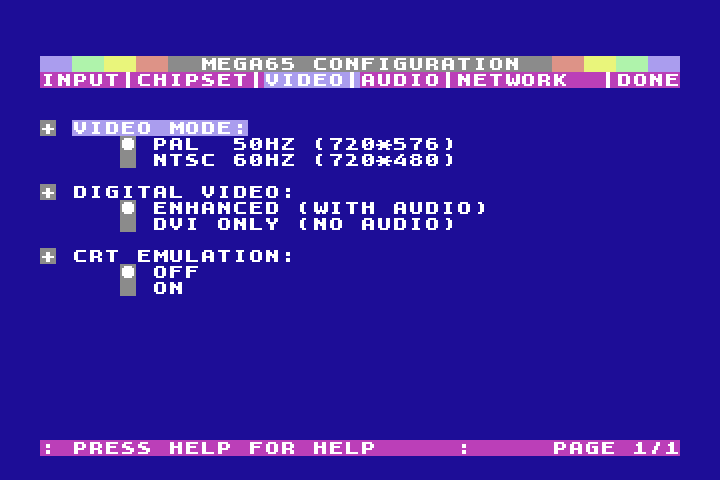
\includegraphics[width=0.7\linewidth]{images/ss-m65config-3.png}
\end{center}

Met {\bf Video mode} kiest u tussen de PAL-compatibiliteitsmodus en de NTSC-compatibiliteitsmodus. U kunt deze instelling ook tijdens het uitvoeren van programma's wijzigen met het Freezer-menu.

Met de instelling {\bf Digital Video} schakelt u het gecombineerde video- en audiosignaal over de Digital Video-poort in of uit. Indien uw Digital Video-beeldscherm ingebouwde luidsprekers heeft, schakelt u deze instelling in ({\bf Enhanced (with audio)}) om deze te gebruiken. Sommige DVI-beeldschermen zonder ingebouwde luidsprekers vereisen dat deze instelling wordt uitgeschakeld.

{\bf CRT emulation} is een optionele instelling die het beeld meer laat lijken op dat van een klassiek beeldbuismonitor wanneer u een modern plat beeldscherm gebruikt.

\subsection{Audio}
\index{Configuratie!Audio}

Op de bladzijde {\bf Audio} stelt u het geluidssysteem van de MEGA65 in.\index{Configuratie!Audio} In de meeste gevallen kunt u deze instellingen op hun standaardwaarden laten staan.

\begin{center}
  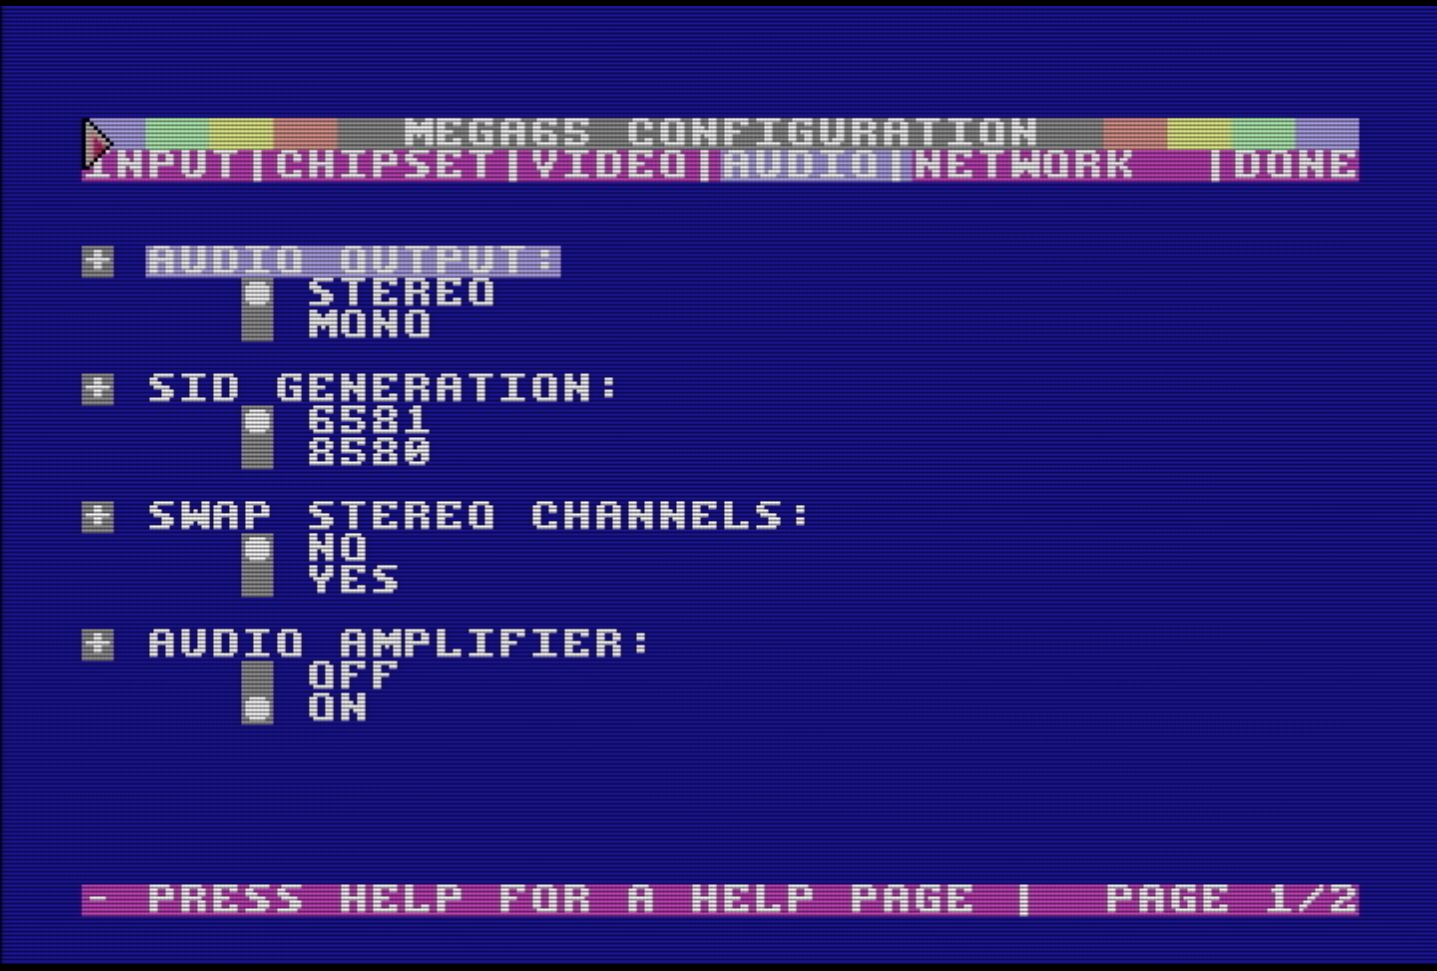
\includegraphics[width=0.7\linewidth]{images/ss-m65config-4.png}
\end{center}

{\bf Audio output} kan worden ingesteld op volledige stereo of op het verzenden van een monauraal signaal naar beide luidsprekers. In de stereomodus kunt u de diverse audioapparaten van de MEGA65 met de audiomixer in het Freezer-menu naar links of rechts in het stereobeeld verplaatsen. De standaardinstellingen plaatsen de vier SID-chips enigszins naar links en rechts.

{\bf SID generation} kiest tussen de audio-emulatie van de twee modellen SID-geluidschips: de oorspronkelijke 6581 die in sommige Commodore 64's wordt gebruikt en de nieuwere 8580 die in latere Commodore 64's en 128's wordt gebruikt. Sommige Commodore 64-spellen maakten gebruik van gebreken in de 6581 die in de 8580 zijn opgelost en klinken daardoor beter met de oudere generatie.

{\bf Swap stereo channels} laat de linker- en rechterluidsprekers van elkaar verwisselen.

{\bf Audio amplifier} regelt de ingebouwde versterker op de 3.5 mm-audioaansluiting. Stel deze in op {\bf on} wanneer u een hoofdtelefoon of een ander apparaat gebruikt dat een versterkt signaal verwacht. Stel deze in op {\bf off} voor een signaal op lijnniveau.

\subsection{Network}
\index{Configuratie!Netwerk}

Op de bladzijde {\bf Network} kunt u het MAC-adres van de ethernetpoort aanpassen. De MEGA65 heeft geen door de hardware toegewezen MAC-adres. In plaats daarvan gebruikt de computer de hier ingevoerde waarde.

Indien het MAC-adres geheel uit nullen bestaat, drukt u op de toets \megakey{R} om een willekeurig adres te genereren. Met een MAC-adres dat geheel uit nullen bestaat, werken netwerkfuncties niet.\index{Configuratie!MAC-adres}\index{Netwerk!MAC-adres}

\begin{center}
  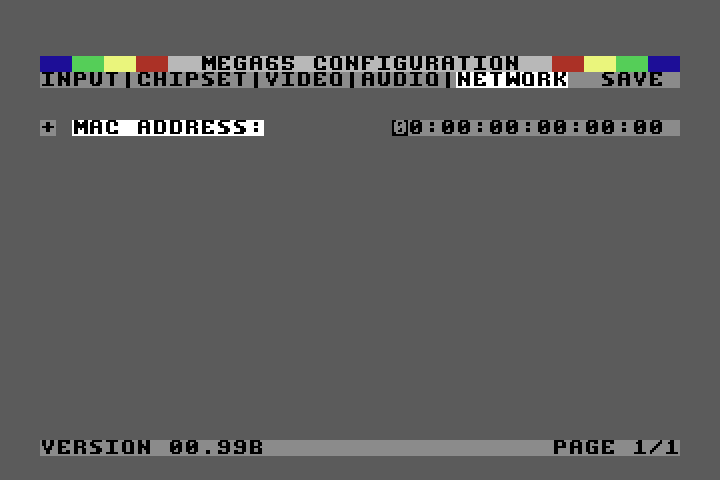
\includegraphics[width=0.7\linewidth]{images/ss-m65config-5.png}
\end{center}

\subsection{Done}

Op de bladzijde {\bf Done} kunt u het Configuratiehulpprogramma verlaten. Indien u wijzigingen hebt aangebracht die u wilt behouden, selecteert u {\bf Save as defaults and exit.} U kunt de wijzigingen ook verwerpen, de fabrieksinstellingen herstellen of volledig opnieuw opstarten naar het scherm van de initiële configuratie.

\begin{center}
  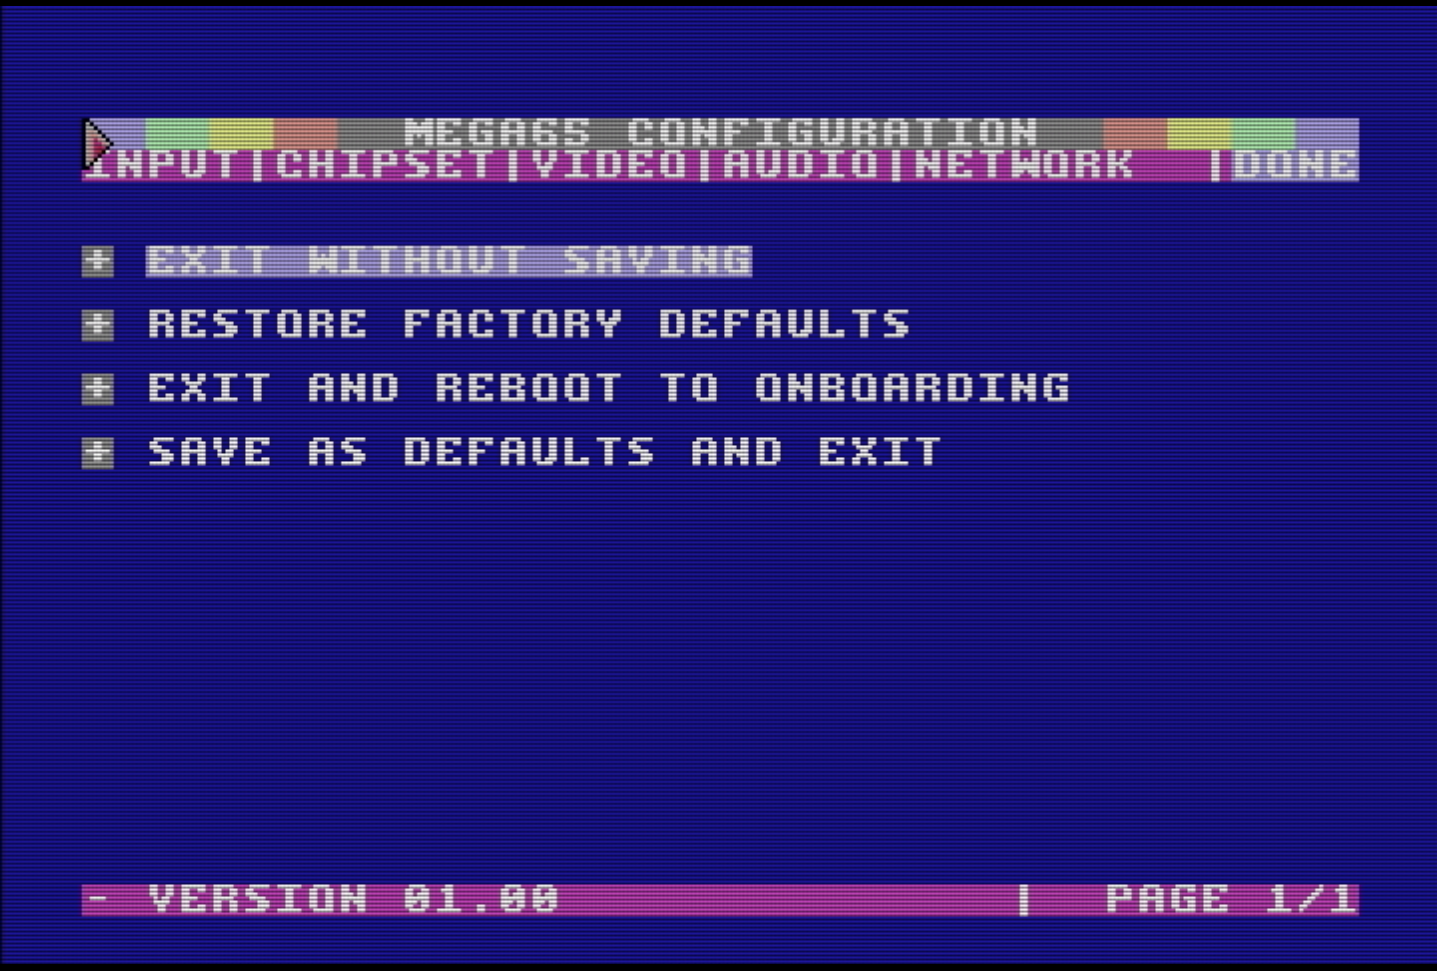
\includegraphics[width=0.7\linewidth]{images/ss-m65config-save.png}
\end{center}

Wanneer u het Configuratiehulpprogramma verlaat, wordt u gevraagd de computer uit en weer in te schakelen. Schakel de computer uit en vervolgens weer in.

\section{Kennismaken met SD-kaarten}
\label{sec:introducing-sd-cards}
\index{SD-kaarten}
\nopagebreak
Uw MEGA65 is uitgerust met twee SD-kaartsleuven: een SD-kaartsleuf op vol formaat in de behuizing, bereikbaar via de onderzijde van de computer, en een microSD-kaartsleuf aan de achterzijde van de computer.\index{SD-kaarten!Locaties} De MEGA65 gebruikt de SD-kaart voor het opslaan van configuratie-instellingen, het laden van het besturingssysteem, het bijwerken van de firmware en het opslaan van uw programmatuur en gegevens als virtuele schijfimages.

De MEGA65 wordt geleverd met een SD-kaart op vol formaat in de interne SD-kaartsleuf, vooraf gevuld met de bestanden van het besturingssysteem en de meegeleverde programmatuur.\footnote{U kunt de oorspronkelijke inhoud van de SD-kaart opnieuw aanmaken met bestanden die u van het internet kunt downloaden. Desondanks wilt u wellicht een reservekopie van de inhoud van de SD-kaart op uw PC maken.} U kunt uw MEGA65 aansluiten en er direct mee beginnen, zonder een nieuwe SD-kaart in te stellen. U kunt deze SD-kaart op zijn plaats laten en doen alsof hij er niet is, alsof uw MEGA65 een computer uit de jaren negentig is met een verborgen mogelijkheid om niet-vluchtige gegevens op te slaan.

De MEGA65 gebruikt slechts één van de twee SD-kaartsleuven tegelijk. Indien er een microSD-kaart in de sleuf aan de achterzijde zit, wordt de interne SD-kaart genegeerd. Welke sleuf u gebruikt, hangt af van het beoogde gebruik van de computer. Naarmate u meer vertrouwd raakt met uw MEGA65, wilt u de SD-kaart wellicht tussen de MEGA65 en uw PC verplaatsen om bestanden te kopiëren en systeemupdates uit te voeren. Dit is gemakkelijker met de externe microSD-kaartsleuf.

U kunt uw MEGA65 ook met een ethernetkabel op uw PC of het plaatselijke netwerk aansluiten en met een hulpprogramma bestanden tussen de twee computers overbrengen. De bestandsoverdrachtfunctie heeft toegang tot de bestanden op de SD-kaart en gebruikt de sleuf die op dat moment actief is. Zie voor meer informatie over het overbrengen van bestanden hoofdstuk \vref{cha:transferring-files}.

\section{Een nieuwe SD-kaart voorbereiden}

U kunt de microSD-kaartsleuf aan de achterzijde van de MEGA65 gebruiken als permanente opslagruimte voor de configuratie- en systeembestanden van de computer. Een voorbereide kaart in deze sleuf heeft voorrang op de SD-kaart die in de computer is geïnstalleerd. Het is handig om een microSD-kaart geïnstalleerd te hebben indien u de kaart tussen uw MEGA65 en uw PC wilt verplaatsen.

De volgende aanwijzingen gelden voor geheugenkaarten in zowel de externe microSD-kaartsleuf als de interne SD-kaartsleuf op vol formaat.

De MEGA65 ondersteunt SD-kaarten van het type SDHC, met een grootte tussen 4GB en 32GB. Oudere kaarten kleiner dan 4GB en nieuwere SDXC-kaarten groter dan 32GB zullen naar verwachting niet werken.

Een SD-kaart moet vóór gebruik door de MEGA65 worden voorbereid met behulp van het SD-kaarthulpprogramma.\index{SD-kaarthulpprogramma} Het hulpprogramma maakt twee partities aan: een verborgen partitie voor configuratiegegevens en freezergegevens en een FAT32-compatibele partitie voor schijfimages en systeembestanden. U kunt toegang krijgen tot de FAT32-partitie door de SD-kaart op uw PC aan te sluiten.\footnote{Indien u een reservekopie van de volledige SD-kaart inclusief de verborgen partitie wilt maken, moet u een schijfhulpprogramma gebruiken dat volledige partities kopieert en niet alleen de bestanden op de FAT32-partitie.}

Een SD-kaart die door een andere computer is geformatteerd, werkt {\em niet} met de MEGA65, zelfs indien die computer alleen de FAT32-partitie wist. U {\em moet} de SD-kaart formatteren met het SD-kaarthulpprogramma van de MEGA65.

\subsection{De SD-kaart plaatsen}

Het formatteren van een SD-kaart wist de inhoud en deze handeling kan niet ongedaan worden gemaakt. Wij raden u aan de interne SD-kaart die bij de computer is geleverd niet te wissen.

Het SD-kaarthulpprogramma vraagt u welke van de kaarten die momenteel in de computer zijn geplaatst, geformatteerd moet worden. U kunt er als voorzorgsmaatregel voor kiezen de interne SD-kaart te verwijderen voordat u het SD-kaarthulpprogramma opent. U kunt hem later opnieuw plaatsen of hem uit de computer laten totdat u hem nodig hebt. Dit is tevens een goede gelegenheid om de gebundelde softwarebestanden (met bestandsnamen die eindigen op {\tt .D81}) van de interne SD-kaart naar uw PC te kopiëren, zodat u ze later op de nieuwe SD-kaart kunt kopiëren.

Het hulpprogrammamenu is toegankelijk, zelfs indien er geen geldige SD-kaart aanwezig is. U kunt een nieuw systeem opstarten met uitsluitend een geschikte SD-kaart en het SD-kaarthulpprogramma.

Plaats de SD-kaart die u wilt voorbereiden, voordat u verdergaat.

\subsection{Het SD-kaarthulpprogramma}
\index{SD-kaarthulpprogramma}

U opent het SD-kaarthulpprogramma vanuit het hulpprogrammamenu.\index{Hulpprogrammamenu} Schakel de MEGA65 uit, houd de toets \specialkey{ALT} ingedrukt en schakel hem weer in. Selecteer in het menu optie \megakey{2} om het SD-kaarthulpprogramma te starten (\texttt{SDCARD FDISK+FORMAT UTILITY}).

\begin{center}
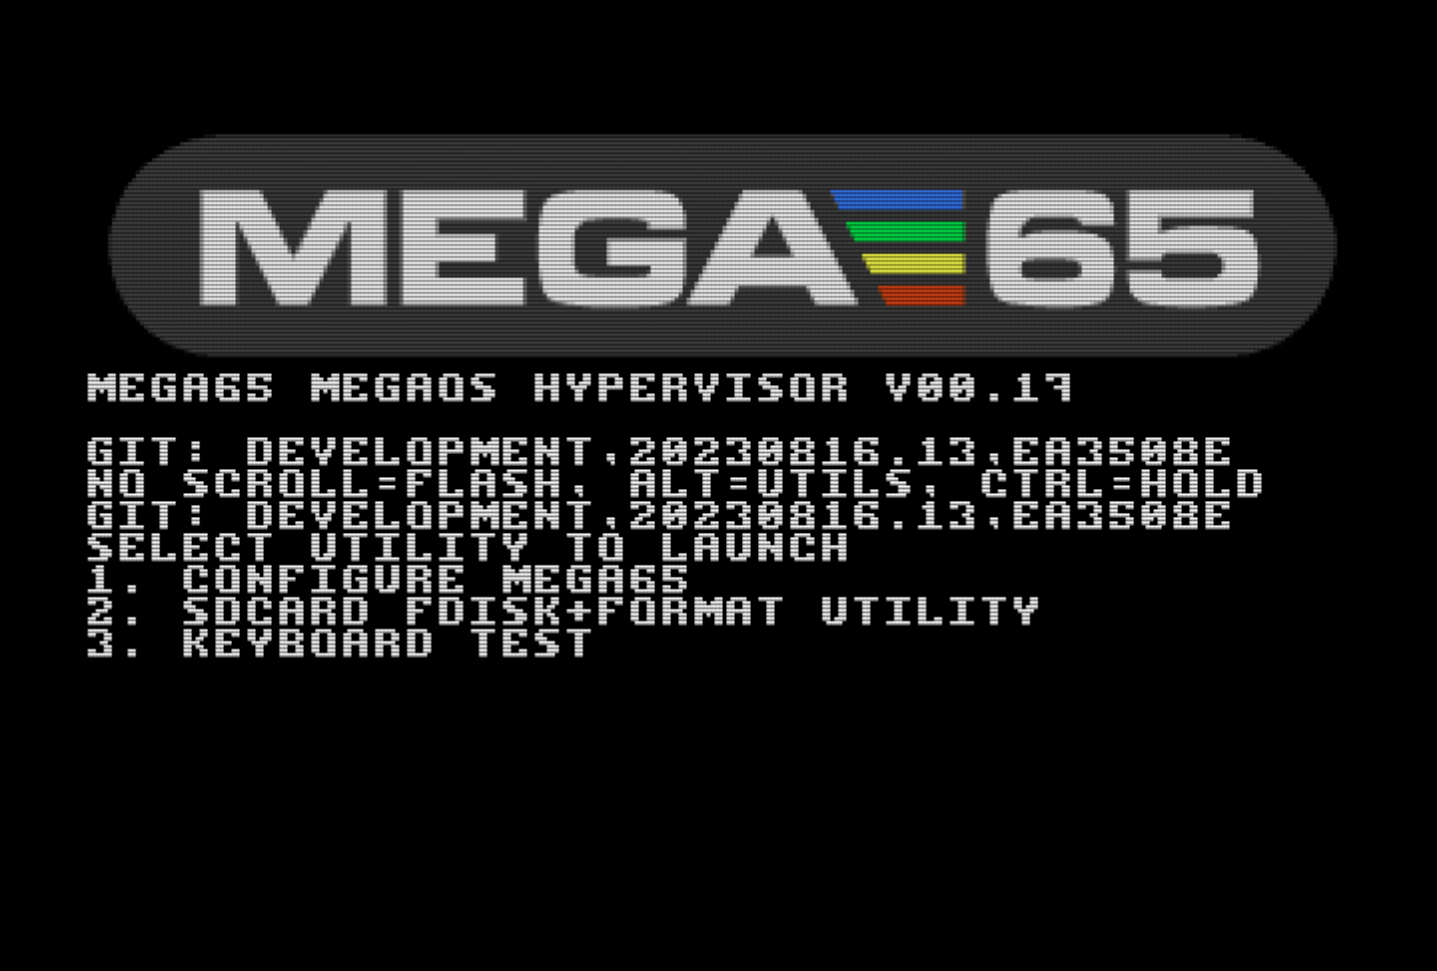
\includegraphics[width=0.7\textwidth]{images/ss-utilmenu.png}
\end{center}

Het SD-kaarthulpprogramma opent en zoekt naar SD-kaarten die in de sleuven zijn geïnstalleerd. Indien u de SD-kaart die u wilt voorbereiden nog niet hebt geplaatst, doe dat nu en druk daarna op \megakey{R} om opnieuw te scannen.

\begin{center}
  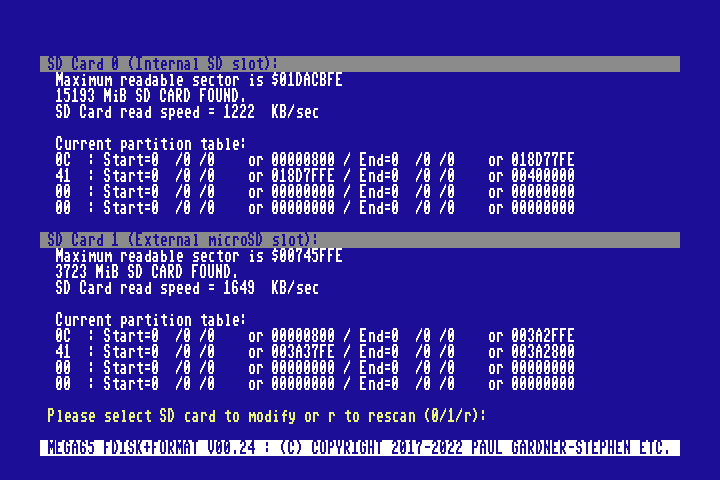
\includegraphics[width=0.7\textwidth]{images/ss-m65fdisk-busselect.png}
\end{center}

Selecteer de kaart die u wilt voorbereiden: \megakey{0} voor de interne SD-kaart, \megakey{1} voor de externe microSD-kaart. Indien er twee kaarten zijn geïnstalleerd, {\em let er goed op dat u de juiste kaartsleuf kiest.}

Het SD-kaarthulpprogramma vraagt bevestiging voordat de SD-kaart wordt gewist. Als allerlaatste voorzorgsmaatregel moet u de tekst {\tt DELETE EVERYTHING} in hoofdletters typen en vervolgens op \specialkey{RETURN} drukken om door te gaan. (Indien u dit proces wilt afbreken, is het veilig om de MEGA65 op dit moment uit te schakelen.)

\begin{center}
  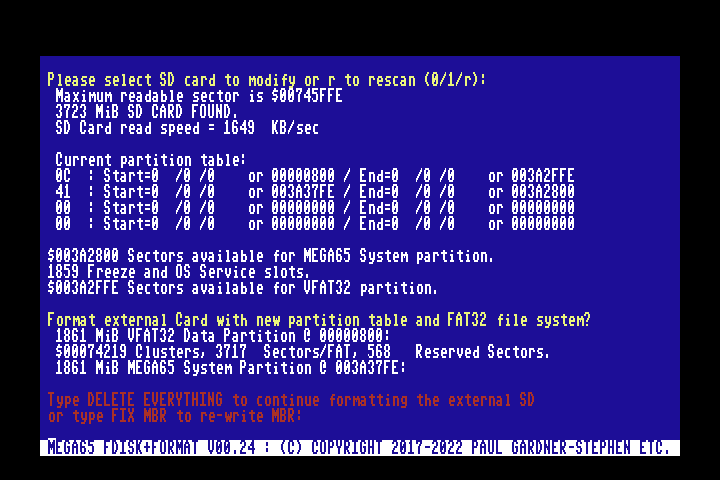
\includegraphics[width=0.7\textwidth]{images/ss-m65fdisk-typesomething.png}
\end{center}

Het hulpprogramma wist de SD-kaart en maakt de partities aan. Wanneer het klaar is, vraagt het of u de systeembestanden wilt installeren. De systeembestanden (met bestandsnamen die eindigen op {\tt .M65} en {\tt .ROM}) zijn in de core ingebed en worden naar de FAT32-partitie gekopieerd voor gebruik. Indien u een bijgewerkte MEGA65-core in slot 1 hebt geïnstalleerd, selecteert u deze; selecteert u anders de in de fabriek geïnstalleerde MEGA65-core in slot 0. (Indien u uw MEGA65 zojuist hebt ontvangen, is slot 0 de enige optie.)

\begin{center}
  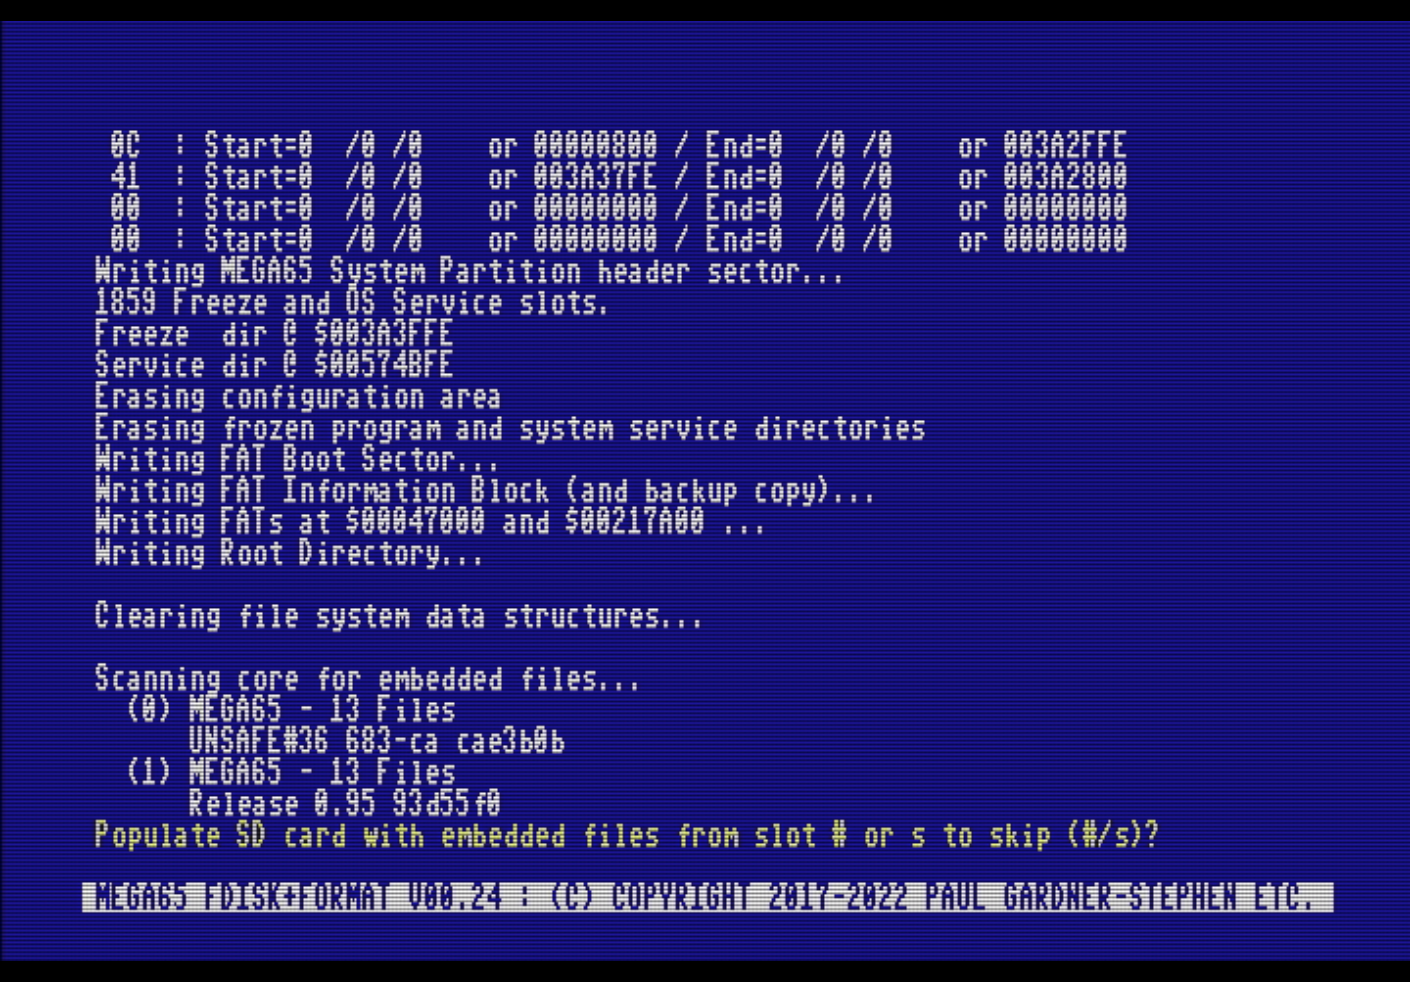
\includegraphics[width=0.7\textwidth]{images/ss-m65fdisk-populate.png}
\end{center}

Start de computer opnieuw op wanneer daarom wordt gevraagd.\footnote{Indien u een core selecteert die {\tt MEGA65.ROM} niet als één van de ingebedde bestanden bevat, vraagt het hulpprogramma u de SD-kaart naar uw PC te verplaatsen om dit bestand erop te kopiëren. Dit gebeurt alleen wanneer u een MEGA65-core gebruikt die afkomstig is van een andere bron dan een officieel MEGA65-releasespakket. Zie voor meer informatie over cores en het verkrijgen van {\tt MEGA65.ROM} hoofdstuk \vref{cha:cores}.}

\subsection{De gebundelde programmatuur verkrijgen}

De systeembestanden die naar de vers geformatteerde SD-kaart worden gekopieerd, omvatten niet de gebundelde programmatuur die bij de oorspronkelijke SD-kaart in de interne kaartsleuf werd meegeleverd. U kunt deze bestanden met uw PC van de oorspronkelijke SD-kaart kopiëren en ze daarna op de nieuwe SD-kaart kopiëren.

De website MEGA65 Filehost\index{Filehost-website} biedt allerlei bestanden aan die u voor uw MEGA65 kunt downloaden. Dit omvat de nieuwste versies van de platformcomponenten, alternatieve cores en honderden spellen, demo's en toepassingen die door de MEGA65-gemeenschap zijn gemaakt. Dit omvat tevens de gebundelde programmatuur van de oorspronkelijke SD-kaart die bij de computer werd meegeleverd.

Indien u de gebundelde softwarebestanden niet meer hebt, kunt u ze verkrijgen via de website MEGA65 Filehost. Bezoek de volgende URL:

\url{https://files.mega65.org/?id=all-intros-public}
